\documentclass{article}
\usepackage{listings}
\usepackage{xcolor}

\lstset{
    language=Python, % 使用する言語
    basicstyle=\ttfamily\small, % フォントの設定
    keywordstyle=\color{blue}\bfseries, % キーワードのスタイル
    commentstyle=\color{green!40!black}, % コメントのスタイル
    stringstyle=\color{orange}, % 文字列のスタイル
    numbers=left, % 行番号の表示位置
    numberstyle=\tiny\color{gray}, % 行番号のスタイル
    stepnumber=1, % 行番号のステップ
    breaklines=true, % 行が長い場合に自動改行するかどうか
    frame=single, % コードブロックに枠を表示するかどうか
    showstringspaces=false, % スペースを文字列に含めるかどうか
    captionpos=b % キャプションの位置
}
\usepackage[margin=1in]{geometry} 
\usepackage[dvipdfmx]{graphicx}
\usepackage{natbib}
\usepackage{url}

\begin{document}

\title{G-coordinator: G-code生成の新たな手法とその可能性}
\author{谷口朝洋*}
\maketitle

\begin{center}
  \large
  G-coordinator: A New Method of G-code Generation and Its Possibility
  
  Tomohiro TAGUCHI
\end{center}

\affil{大阪府立大学 工学域 機械系学類 \\ 機械工学課程 機械力学研究室 \\ 〒599-8531 大阪府堺市中区学園町 1-1}



\section*{Abstract}
This study focuses on the development of a novel method for generating G-code, the program read by a 3D printer. 
We have developed an open-source software called G-coordinator, 
which utilizes Python and mathematical functions to create G-code directly and construct three-dimensional shapes. 
This alternative path generation technique, which is distinct from traditional slicing methods, 
offers the potential to tackle complex shapes that were previously challenging to produce 
and enables the formation of more precise printing conditions and paths. 
It also facilitates the straightforward realization of mathematical shapes.\\
\textgt{keywords}: \keywords{G-code, 3D Printing, Python, Open-source}

\section*{要旨}
本研究は,MEX型3Dプリンタを用いて造形を行う際に,機械に読み込ませるプログラムであるG-codeの新たな生成方法に関するものである.
Pythonと数学的な関数を用いてG-codeそのものを直接作成し,3次元形状を構築することできるG-coordinator 
( https://github.com/tomohiron907/G-coordinator )というオープンソースソフトウェアを開発した.
従来の「スライス」とは異なる手法によるパス生成により,より精密な印刷条件の調整が可能になるとともに,
いままでは難しかった形状や,数理的な形状の容易な実現が期待できる.
本論文では,G-coordinatorの特徴を述べるとともに,その造形方法やgcoordinatorライブラリを用いた実装方法についてその概要を述べる.
また,それらの技術を用いた具体的なユースケースについても詳述する.\\
\textgt{キーワード}: \keywords{G-code, 3D プリント, Python, オープンソース}


\begin{twocolumn}

\section{はじめに}
\subsection{G-coordinatorとは}
G-coordinatorは,Pythonを用いて3Dプリンタ用G-codeを生成できるソフトウェアである.
従来のスライスソフトによるG-code生成と異なり,造形から印刷条件の調整まで3Dプリントに必要な工程の全てをG-coordinatorひとつで完結させることができる.
Windows, Macに対応したGUIアプリケーションに加えて,Python用のライブラリも公開している.
どちらもPythonを用いて造形と印刷条件の設定を行うが,GUIアプリに関しては,Python環境を整える必要がなく,誰でも簡単にG-codeを生成することができる.
Figure\ref{fig:1}にG-coordinator(GUIアプリ)のスクリーンショットを示す.G-codeを書き出す手順は主に4つのステップから構成される.
\begin{enumerate}
  \item コードを書いて,造形を決定
  \item グラフィックスビューで詳細を確認
  \item 印刷条件の設定
  \item G-codeの出力
\end{enumerate}

\begin{figure*}[h]
  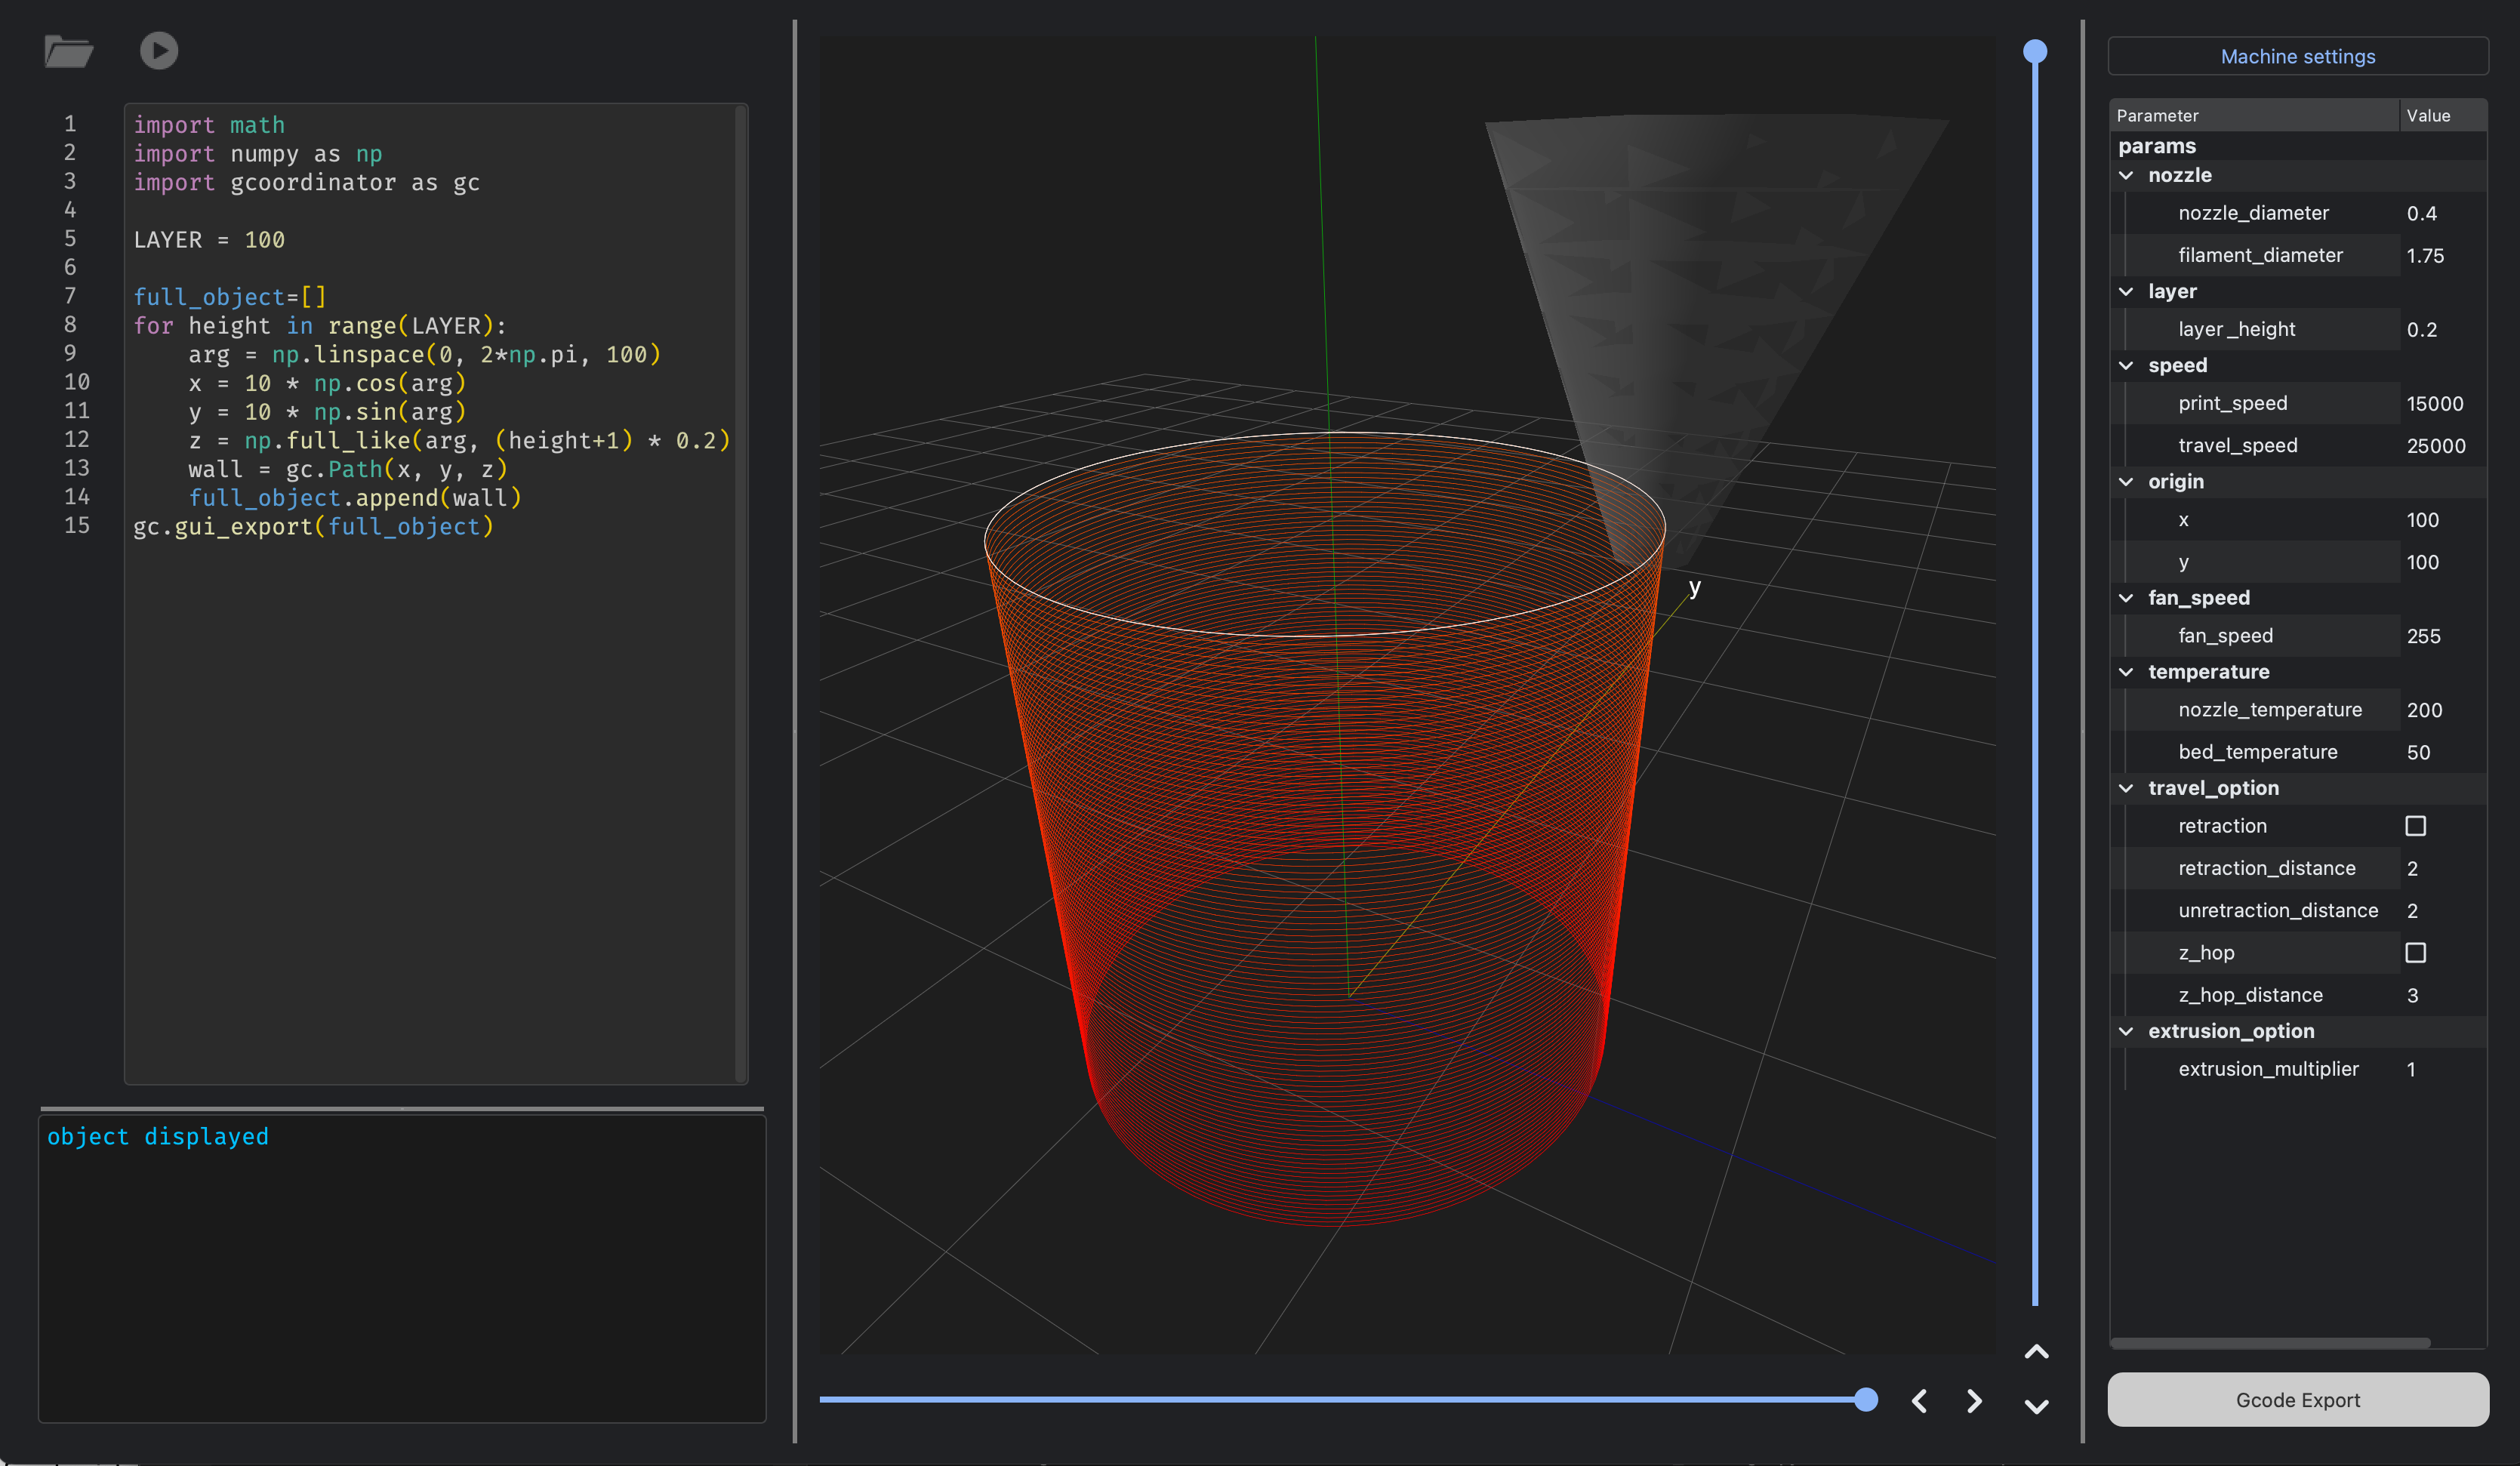
\includegraphics[width=\linewidth]{img/screenshot.png}
  \caption{screenshot of G-coordinator}
  \label{fig:1}
\end{figure*}
  
\subsection{背景}
一般的に,3Dプリンタを用いる際にはCAD等で3Dデータを作成し,その3Dデータをスライスソフトで処理し,G-codeを生成する.
スライスソフトは,3Dプリンタのノズルパスを自動で算出することができ,多くのユーザに取って,より簡単にG-codeを作成することができる.
しかし,より細かい制御やマニュアルでの制御を求めるユーザにとっては,スライスソフトでは3Dプリンタの挙動や印刷設定のマニュアル制御ができない.
そこで,近年,3Dモデルを介さず直接G-codeを作成するG-code Modeling\cite{chinen_thesis}の手法が台頭している.
G-coordinatorは,G-code Modelingの新たな手法として位置付けられる.

\subsection{目的}
本研究は,広範なユーザに向けた高い自由度を有するG-codeモデリングを実現し,
これにより従来のCADやスライサでは到達できなかった造形を具現化することを目的としている.
G-coordinatorにより,3Dプリントにおける新たな可能性が開かれ,現行の技術では実現が難しい形状や構造の物体を容易に製造することが可能となる.

\subsection{G-codeとは}
G-codeは,コンピュータ制御された機械操作を指示するための標準的なプログラミング言語であり,
その本質はツール(MEX型3Dプリンタにおいてはノズル)の位置を記述する座標列にある.
G-codeの基本的な構造は,各行においてツールの移動先の座標が指定され,これによってツールの位置が制御される.
たとえば,以下は一般的なG-codeの例である.
\begin{verbatim}
G1 F1000 X100 Y80 Z0.4 E0.5 
\end{verbatim}
このコマンドで,機械はノズルを(X, Y, Z) = (100, 80, 0.4)の座標に1000mm/minの速さで移動させながらフィラメントを0.5mm送る.
これらのコマンドが,G-codeの内部では,数百から数万行繰り返される.
G-codeには印刷速度やフィラメント送り量など様々な要素があるものの,これらは,ソフトウェアで自動的に決定できるため,
G-code Modelingにおいてユーザはノズルの移動する座標列のみを考慮すれば良い. 

ここで,上記のG-codeの性質から,G-coordinatorでのモデリングに不可欠な二つの用語を定義する.
\begin{itemize}
  \item セグメント:ノズルが移動する最小単位の線分.
  \item パス:樹脂が連続的に押し出されてできる一本の経路.
\end{itemize}

Figire\ref{fig:2}は,6角形のパスが下から積層されており,一番上のパスの最初のセグメントまでが表示されている.
このように,セグメントが集まってパスになり,パスが集まってひとつの造形物になる.


\begin{figure}[htbp]
  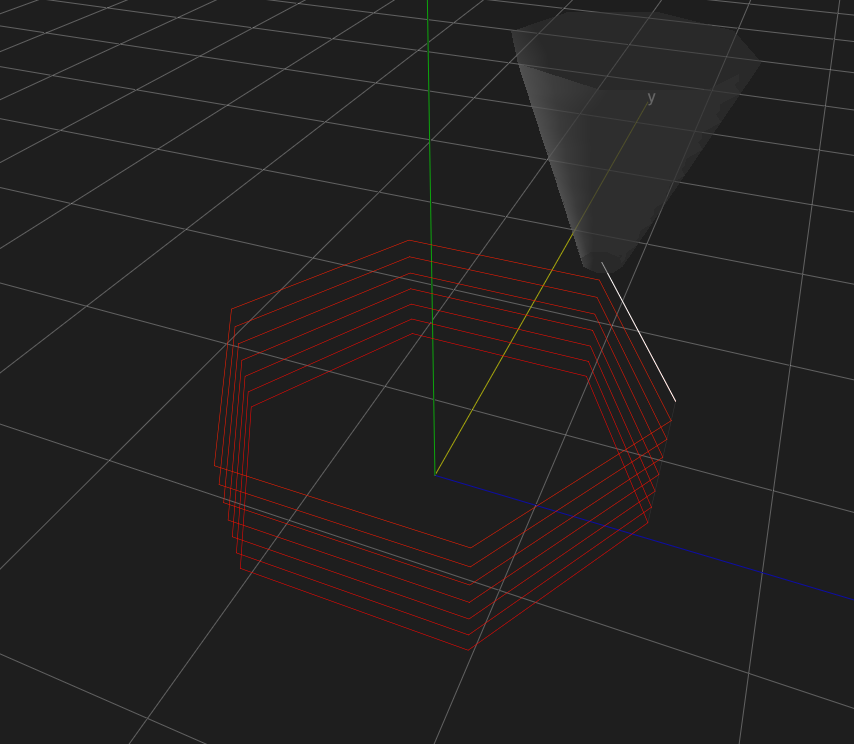
\includegraphics[width=\linewidth]{img/path_segment.png}
  \caption{path and segment}
  \label{fig:2}
\end{figure}

\section{関連研究}
現代の3Dプリントにおいて,G-code Modeling の手法としてRhinocerosとそのプラグインGrasshopperやFullcontrolGCodeDesignerなどが広く利用されている.
本章では,これらの手法とG-coordinatorとの比較に焦点を当て,それらの特徴と差異を明らかにする.
\begin{table*}
  \centering
  \caption{ソフトウェアの比較}
  \label{table:software_comparison}
  \begin{tabular}{|c|c|c|c|c|c|}
    \hline
    \textbf{ソフトウェア} & \textbf{オープンソース} & \textbf{拡張性} & \textbf{多軸印刷} & \textbf{インフィル} & \textbf{スキル要求} \\
    \hline
    Rhino+GH & $\times$ & $\bigcirc$ & $\triangle$ & $\triangle$ & 低 \\
    \hline
    FullControl & $\bigcirc$ & $\triangle$ & $\times$ & $\times$ & 低 \\
    \hline
    G-coordinator & $\bigcirc$ & $\bigcirc$ & $\bigcirc$ & $\bigcirc$ & 高 \\
    \hline
  \end{tabular}
\end{table*}

\subsection{Rhino+Grasshopper}
RhinocerosとそのプラグインGrasshopperの組み合わせは,G-code Modelingの代表的な手法の一つであり,その特徴は以下の通りである.\\
オープンソース: 非公開\\
拡張性: 有り\\
多軸制御: 有り\\
インフィル: 一部制限あり\\
要求スキル: 低い\\
Rhino+Grasshopperはオープンソースではないが,アドオンやプラグイン等の拡張性は高く,
多軸制御やインフィルに関してはアドオンで実現できるものも多い.
また,プログラミングの形式がビジュアルプログラミングであることから,プログラミングに慣れていないユーザにも扱いやすいソフトウェアと言える.
しかし,ソフトウェアの値段が比較的高価であり,一般の利用者は容易にそのソフトウェアを試用することが難しい状況にある.

\subsection{FullControlGCodeDesigner}
FullContolGcodeDesinger\cite{gleadall2021fullcontrol}は,Excel上で動作するマクロとしてのソフトウェアである.\\
オープンソース: 公開\\
拡張性: 制限あり\\
多軸制御: 非対応\\
インフィル: 非対応\\
要求スキル: 低い\\
FullContolGcodeDesingerはオープンソースであるが,拡張性には限りがあり,多軸制御やインフィルの生成には対応していない.
Excelシートであるため,新たなソフトをインストールする必要がなく,初めG-code Modelingを行うユーザに向いているが,
Excelのみで造形を完成させる性質上,複雑な形状や関数の扱いには限界がある.
また,その点を克服したpythonライブラリ,fullcontrolも登場しているが,python環境をユーザが整える必要があるなどの弱点もある.

\subsection{G-coordinator}
G-coordinatorは,G-code Modelingの新しい手法であり,以下がその特徴である.\\
オープンソース: 公開\\
拡張性: 有り\\
多軸制御: 有り\\
インフィル: 有り\\
要求スキル: 高い\\
G-coordinatorはオープンソースであり,あらゆるコードやライブラリを公開している.
拡張性に優れ,Pythonを用いた造形により,様々なデータソースを活用可能である.
多軸制御やインフィルの生成にも対応している.
しかしながら,G-coordinatorでの造形には多少の数学的知識とコードのスキルを要求してしまう側面がある.
これらの特徴により,G-coordinatorはG-code Modelingの新たな展開を可能にしており,従来の手法と比較して優れた柔軟性と拡張性を提供している.

\section{実装}
\subsection{G-coordinatorの造形方法}
G-coordinatorで造形を行うための方法を,最も簡易な円柱モデルを用いて述べる.
なお,円柱壁の造形コードを補足資料に掲載している.いかに複雑な形状であっても,基本的な造形のプロセスは同じである.
G-coordinatorでは,パスのx, y, z座標列を計算して,それらの座標列からPathオブジェクトを作成する.
より詳細な造形コードの作成に関してはG-coordinator公式ドキュメントを参照されたい.
\subsubsection{円形パスの生成}
円柱は円形のパスが縦に造形されたものであることから,まず円形のパスを生成する.

\begin{lstlisting}
  import numpy as np
  import gcoordinator as gc
  full_object = []
\end{lstlisting}

まず,numpyライブラリ,gcoordinatorライブラリをインポートする.
次に,full\_objectという空のリストを作成する.
これは,後にPathオブジェクトを格納するためのものである.

\begin{lstlisting}
  arg = np.linspace(0, 2*np.pi, 100)
  x = 10 * np.cos(arg)
  y = 10 * np.sin(arg)
  z = np.full_like(arg, 0.2)
\end{lstlisting}

円を造形するので,0から2πまでの項数100の角度についての等差数列
(arg)を作成し,その角度のcos, sinがそれぞれx, y座標列になる.
z座表列に関しては,argと同じ項数で,値が0.2(レイヤー厚さ)である数列を用意すればいい.

\begin{lstlisting}
  wall = gc.Path(x, y, z)
  full_object.append(wall)
  gc.gui_export(full_object)
\end{lstlisting}

x, y, z座標列を引数として,Pathオブジェクトのインスタンスを生成する.生成したPathオブジェクトをfull\_objectに追加する.
作成したfull\_objectをgui\_export関数に渡すことで,GUI上で確認することができる.

なお,厳密な表現をすれば,上記のコードで作成できるのは円ではなく,正99角形である.
これは,argが0から2πまでで工数が100の等差数列であるから,角度列を順に繋いでできるセグメントは99個存在するからである.
しかし,半径10mmの場合,99分割ほどの段階で,3Dプリントにおいては無視できる程度にセグメントは小さくなる.
もちろん,分割数を大きくすれば,精度は上昇するが,同時に計算時間も大きくなってしまう.
G-codeには,円弧補完のコマンド(G02, G03)があるが,G-coordinatorでは現在は未実装であるので,円を造形する場合はこのような方法で行う.

\subsubsection{円柱の造形}
円柱を造形するには,前節で述べた円形のパスを縦に積み上げていけば良い.
この処理はfor ループを用いて用意に記述できる.
\begin{lstlisting}[breaklines=false]
for height in range(100):
  arg = ...
  x   = ...
  y   = ...
  z = np.full_like(arg, (height+1) * 0.2)
  wall = ...
  full_object.append(wall)
\end{lstlisting}
このforループの中で,heightは0から99まで1ずつ増加する.
x, y座標列は円形パスと同じで,z座標列をheightの値に応じて0.2ずつ大きくすれば良い.
ここで,heightに1を足してから0.2をかけているのは,ループの始めにおいて,heightの値が0の時に,ノズルの高さが0.2にしたいからである.
そして,forループごとにパスオブジェクトを作成し,full\_objectに追加すれば良い.
即ち,full\_objectには,印刷すべきパスが印刷順に100個のパスが格納されている.
円柱を造形するための造形コード全体を付録に載せる.

\subsubsection{パスの変形}
gcoordinatorライブラリのTransform クラスのメソッドを利用することで,作成したパスを変形させることができる.
\begin{itemize}
  \item gc.Transform.move(): パスを平行移動,回転させる
  \item gc.Transform.rotate\_xy(): XY平面上で回転させる
  \item gc.Transform.stretch(): パスを伸縮させる
  \item gc.Transform.offset():  パスを指定した距離だけオフセットさせる

\subsection{個別印刷設定} 
G-coordinatorでは,以下に示す印刷設定を指定することができる.

\begin{enumerate}
  \item nozzle
  \begin{enumerate}
    \item nozzle\_diameter [mm]
    \item filament\_diameter [mm]
  \end{enumerate}
  \item layer
  \begin{enumerate}
    \item layer\_height [mm]
  \end{enumerate}
  \item speed
  \begin{enumerate}
    \item print\_speed [mm/mim]
    \item travel\_speed [mm/mim]
  \end{enumerate}
  \item fan\_speed
  \begin{enumerate}
    \item fan\_speed [0-255]
  \end{enumerate}
  \item temperature
  \begin{enumerate}
    \item nozzle\_temperature [celcius]
    \item bed\_temperature [celcius]
  \end{enumerate}
  \item travel\_option
  \begin{enumerate}
    \item retraction [true/false]
    \item retraction\_distance [mm]
    \item unretraction\_distance [mm]
    \item z\_hop [true/false]
    \item z\_hop\_distance [mm]
  \end{enumerate}
  \item extrusion\_option
  \begin{enumerate}
    \item extrusion\_miltiplier
  \end{enumerate}
\end{enumerate}

G-coordinatorでは,パラメータツリーで設定したグローバルな印刷設定に対して,個別のパスへの詳細設定をコードから指定することができる.

例として,ベッド定着のためにファーストレイヤにおいてのみ,印刷速度を遅くしたいという状況を考える.
作成したPathオブジェクトの属性としてこれらの印刷設定の値を格納できる.
従って,以下のコードをforループの中に追加すれば,ファーストレイヤの印刷速度をマニュアルで指定できる.
\begin{lstlisting}
if height == 0:
  wall.print_speed = 5000
\end{lstlisting}

操作画面右側のパラメータツリーでのprint\_speedの値が10000の時,上のコードを実行すれば,
第0層目(ファーストレイヤ)では印刷則と5000mm/min, 他の層では,10000mm/minとなり,印刷速度の個別制御が実現できる.
印刷速度に限らず,射出係数,リトラクション,z hop,などグローバル設定で指定できる設定値は,全て個別に値をマニュアル調整することができる.

\subsection{G-code}
\subsubsection{G-code出力方法}
前節までの内容で,ノズルが移動する座標列の情報とその時の印刷設定の情報を内部に保持したパスオブジェクトを作成することができた.
本節では,それらのパスからG-codeに変換する方法について述べる.

G-coordinator(GUIアプリ)では,Fig\ref{fig:1}の画面の右下のG-code Exportボタンを押すことで,G-codeを出力することができる.
なお,スタート,エンドG-codeは,画面右上のmachine settignsボタンを押して出てくるポップアップウィンドウで設定することができる.

pythonライブラリのみを使用する場合には,以下のコードを造形コードの最後に追加する.

\begin{lstlisting}
  gcode = gc.GCode(full_object)
  gcode.start_gcode("path/to/start_gcode.txt")
  gcode.end_gcode("path/to/end_gcode.txt")
  gcode.save('your.gcode')
\end{lstlisting}

\subsubsection{G-code出力の内部処理}
座標列とパスに紐づけられた印刷設定の情報をもとにG-codeを生成する手順について述べる.

パスを構成する各セグメントに対して射出量を以下のように計算される\cite{akhoundi2020calculating}:

\begin{equation}
  E_{i}=\frac{4 w h L_{i}}{\pi D^{2}} \cdot k_{i}
\end{equation}

ここで,各文字の意味は以下の通りである.
\begin{itemize}
  \item $E_{i}$: i番目のセグメントの射出量
  \item $D$: フィラメントの直径
  \item $L_{i}$: i番目のセグメントの長さ
  \item $w$: セグメントの横幅(ノズル直径)
  \item $h$: パスの厚み(レイヤー厚さ)
  \item $k_{i}$: i番目のセグメントの射出係数
\end{itemize}



\section{ユースケース}
以下に,G-coordinatorを用いて造形したユースケースを示す.

\subsection{網目テクスチャ}

京都の新工芸舎\cite{shinkogeisha}のTilde\cite{tildeprinted}にインスパイアを受けて作成した作成をFig.\ref{fig:WaveTray}に示す.
ノズルをジグザグに蛇行させ,一層ごとに位相を反転させることで,積層痕を意匠化させた.
スライスソフトでは,直接ノズルパスを編集できないため,テクスチャを付与することが困難であった.

\begin{figure}[htbp]
  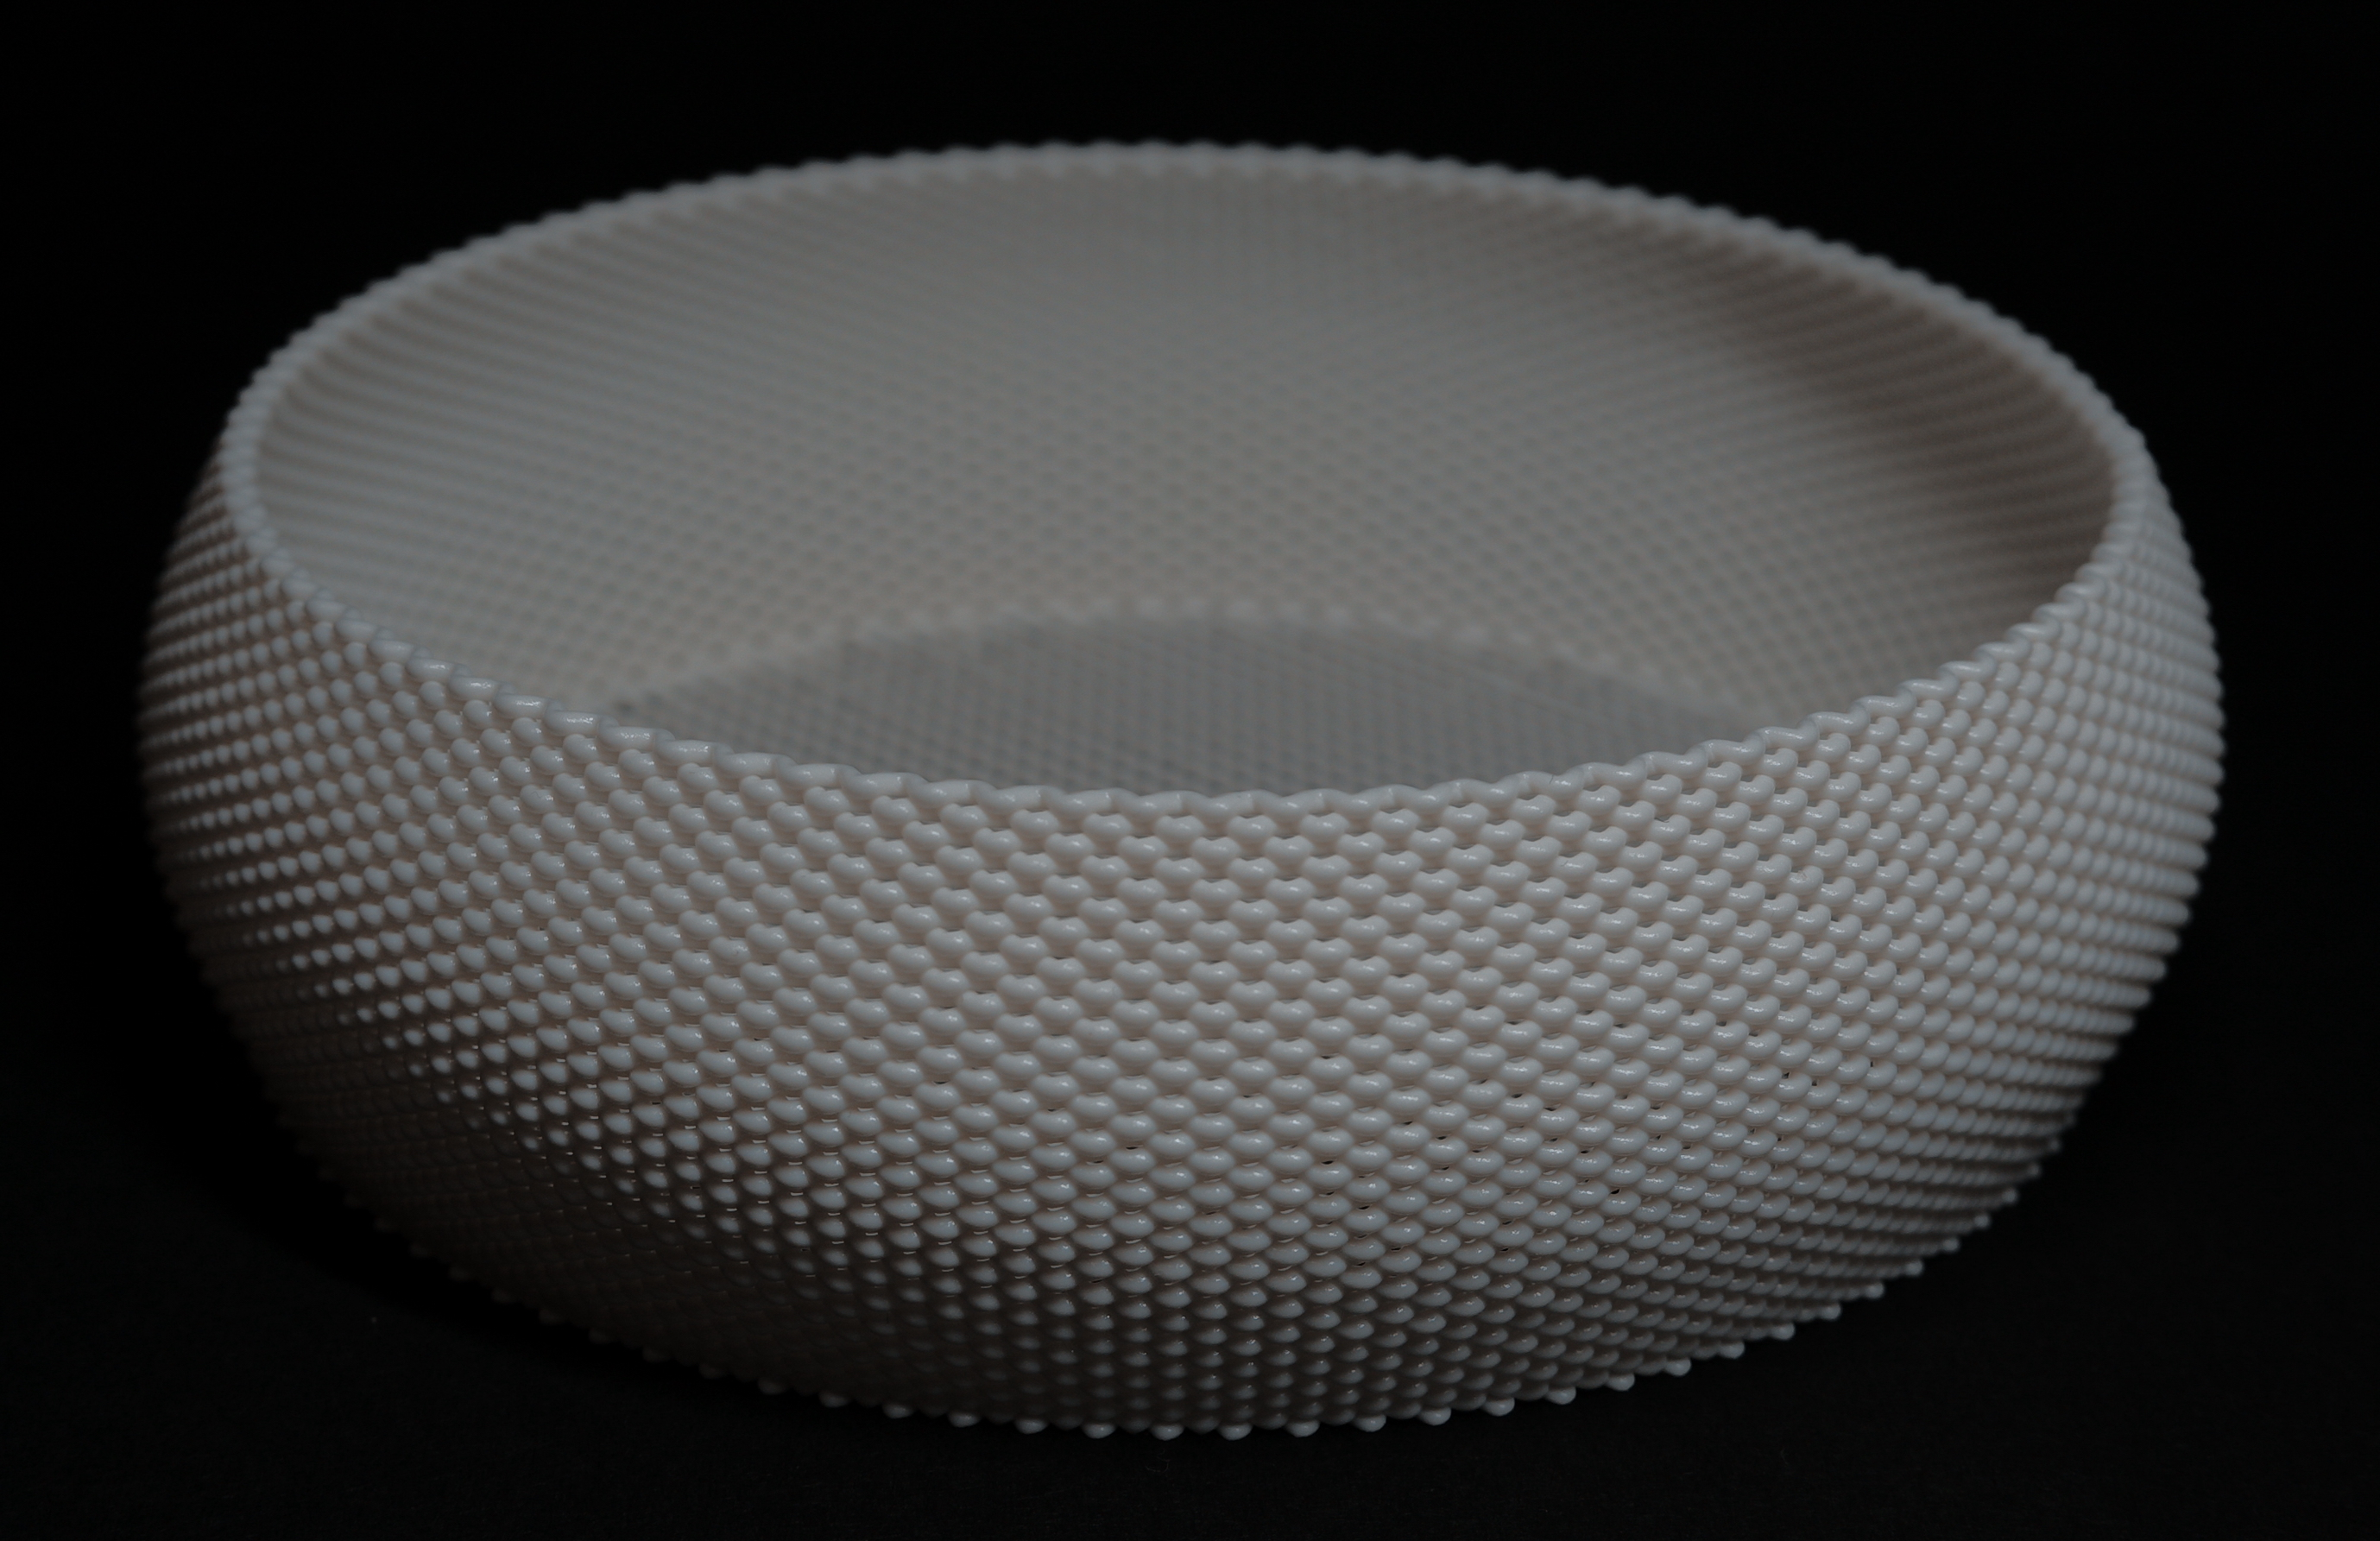
\includegraphics[width=\linewidth]{img/wave_tray.JPG}
  \caption{Woven textured tray}
  \label{fig:WaveTray}
\end{figure}

\subsection{数理的な形状}\label{sec:mathmaticalShape}
G-coordinatorではコードと関数を用いてモデリングを行うため,数理的な形状の実現が極めて容易にできる.
Figure\ref{fig:fractal}は,フラクタル形状を3次元に押し出したもの.他にも,一葉双曲面や,リサージュ曲線を造形するためのコードも公開している.

\begin{figure}[htbp]
  \includegraphics[width=\linewidth]{img/fractal.JPG}
  \caption{koch snowflake pot}
  \label{fig:fractal}
\end{figure}

\subsection{振動による図柄表示}
Pythonの持つ豊富なライブラリを用いれば,あらゆるものをモデリングのために活用できる.
Figure\ref{fig:audrey}は,OpenCVのライブラリを用いて,モノクロ写真から,ある座標でのピクセルの濃さを抽出,その値を振動の振幅に重みとしてかけている.
白のプレートを印刷後,黒の樹脂で振動パターンを印刷している.その結果,ミクロでは不規則な振動が,マクロでは写真に見える状況を実現している.
従来のCADによる造形では,写真を参考にして造形を行うことはできるが,写真データを直接扱うことはできなかった.
pythonを用いて造形を行う恩恵により,いままでよりも多彩なデータソースを扱うことができる.
\begin{figure}[htbp]
  \includegraphics[width=\linewidth]{img/audrey_2.jpg}
  \caption{画像の振動パターン化}
  \label{fig:audrey}
\end{figure}

\subsection{インフィル}
他のG-code Modelingと比較して,G-coordinatorの大きな特徴のひとつとして,Fig.\ref{fig:infill}に示すようなインフィルを利用できることが挙げられる.
インフィルを利用できるようになると,実用性を意識したものを作成することができる.
現在は,line infiil, gyroid infillの二種類を利用可能である.

以下のコードをfor文の中に記述することで,最初の20レイヤーにインフィルを付与することができる.
\begin{lstlisting}
if height<20:
    gyroid = gc.gyroid_infill(wall, infill_distance = 2)
    full_object.append(gyroid)
\end{lstlisting}

ここで,wallオブジェクトは外枠を表すPathクラスのオブジェクトである.
gyroid\_infill関数はインフィルを計算する関数であり,外枠のパスを入力として,その内部を埋めるパスを返す関数である.
ただし,インフィルは一本の曲線で表されるものではなく,複数のパスがまとまって,1レイヤー分のインフィルが構成されているため,
厳密には関数からの返り値として返されるのはPathListクラスのオブジェクトである.
しかし,PathListクラスのオブジェクトもPathクラスと同様に印刷設定の指定などができるため,ユーザはPathオブジェクトと同じように扱うことができ,
そのクラスの違いを大きく意識する必要性は少ない.
\begin{figure}[htbp]
  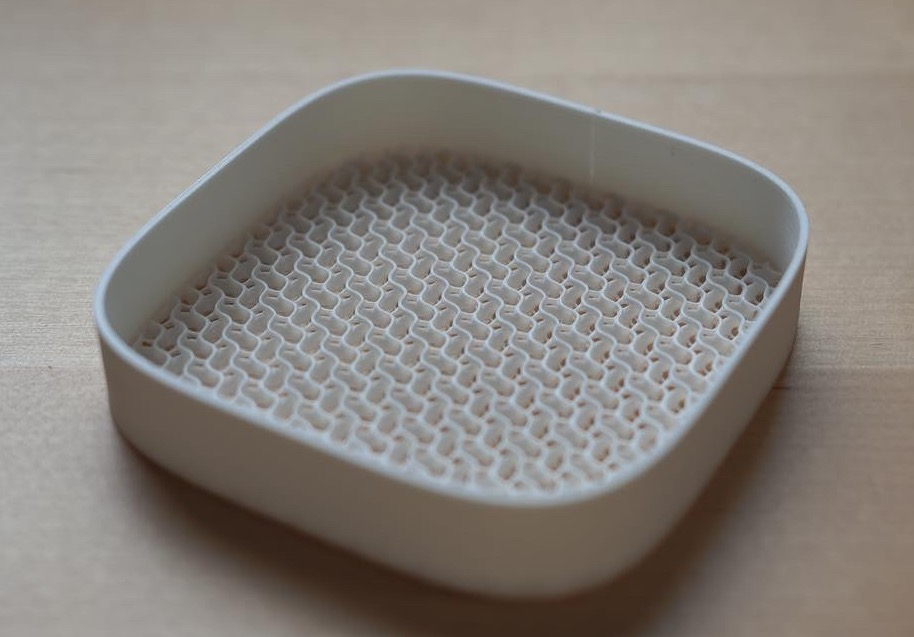
\includegraphics[width=\linewidth]{img/infill_case.JPG}
  \caption{底部にインフィルを付与した小物トレー}
  \label{fig:infill}
\end{figure}

\section{将来展望}
\subsection{開発中のテスト機能}
G-coordinatorを用いて様々な造形を可能にするためにいくつかの機能を開発中である.
何れの機能も既に現在のG-coordinator ver3.0.0にはアルファ版の機能として実装されている,
\subsubsection{数式処理}
\ref{sec:mathmaticalShape}節に示すように,G-coordinatorの機能を利用して数式処理を行うことができる.
現在は,さらにその点を生かすべく,様々な関数やクラスを開発中である.
具体的な例として,陽関数のプロットやパスの生成は容易である一方で,陰関数のプロットは高い難易度を伴う.
この課題に対処するため,numpyのmeshgridを活用し,陰関数によって表現された曲線や曲面をより容易に生成できる枠組みを開発中している.
この取り組みにより,より広範で複雑な数学的表現を容易に扱えるようになり,研究や応用上での有用性が向上することが期待される.

\subsubsection{多軸制御}
多軸3Dプリンタの制御においては,座標に加えてノズルの傾きなど,より複雑な要素が造形プロセスに関与するため,その難易度は著しく高まる.
この課題に対処するため,より使いやすく効果的な多軸造形が可能となるようなフレームワークの開発を進めている.

具体的には,クォータニオン(四元数)を活用したノズルの姿勢制御の開発に焦点を当てている.
現行のG-coordinatorの多軸制御手法では,オイラー角や回転行列を使用して姿勢制御を行っている.
それに対し,クォータニオンを導入することで,ジンバルロックなどの特異点をなくしつつ,より柔軟で安定した姿勢制御が可能となる.\cite{yamaguchi1991}
さらに,計算量が削減され,処理時間が短縮されるという利点もある.

新たな手法による多軸制御G-codeの生成においても積極的に取り組んでおり,これによりユーザがより容易に多軸造形を行える環境を提供することを目指している.

\subsubsection{スライス機能}
G-coordinatorは基本的にすべてコードを用いて造形を行う.
しかし,工業的な形状の造形をコードのみで行うことは難しい.
そこで,G-coordinatorにはstlデータをスライスする関数も用意している.

\begin{lstlisting}
  wall = slice(mesh, height*0.2)
\end{lstlisting}
このように,スライス関数にスライス対象のメッシュとスライスする高さを入力することで,スライスした結果のパス(正確にはPathListオブジェクト)が出力される.
純粋なスライスソフトとは異なり,スライスしたパスに対して,個別の印刷設定をマニュアルで付与することができる.
しかし,現在実装しているスライスアルゴリズムではスライスの計算時間が比較的長いことや,トップ/ボトムの表面を手動で設定しなければならない等の問題もあり,まだ完全な実用段階ではない.
将来的には,前節で述べた多軸制御と絡めて,多軸マシンのためのスライス機能もサポートする予定である.

\subsection{ソフトウェアの開発方針}

G-coordinatorは,数学とコードにより,いままで出来なかった形状を実現する一方で,同時に,
ユーザには多少の数学的知識と,プログラムに関するスキルを要求するものであり,参入のための障壁は比較的高いと言わざるをえない.
そこで,現在想定しているG-coordinatorの将来像は大きく分けて二つある.

一つは,Processingなどを代表とするビジュアルアートを実物化させるためのソフトウェアとしての活用である.
Processingは,プログラムを書いて画面上に図形や形状を描画することができるソフトウェアであるが,
G-coordinatorはプログラムを書いて実際に触れるモノを作成できるソフトウェアである.
これにより,アーティストやデザイナーは数学的なアルゴリズムを用いて,従来不可能だった美しい形状を3Dプリンティングで具現化することが可能になる.

もう一つは,G-coordinatorが数理的な形状に得意な性質を生かし,物理シミュレーションや計算力学を応用して形状を実物化させるソフトウェアとしての利用である.
具体的には,トポロジー最適化のアルゴリズムをG-coordiantorの内部で実装し,最適化計算からG-code生成までをシームレスに行うことができるソフトウェアの実現を目指している.
これにより,エンジニアや科学者は複雑な物理的な現象をシミュレートし,それを具現化するのにG-coordinatorを活用できる.

プログラムを使った3D形状の生成と制御が主眼となる点で,どちらの展望も共通している.

\section{結論}

MEX型3Dプリンタユーザにとって,CAD などの造形手段と,印刷のための調整を行うスライサを同時に置き換える新たな手段としてのG-coordinatorのポテンシャルについて述べた.
スライスソフトに比べて,全部を機械任せにできない欠点はあるものの,裏を返せば,3Dプリンタの挙動の細部までマニュアル操作可能という大きな利点がある.
あらゆる人々に最も自由度の高いG-code Modelingを提供するG-coordiantorは,数学とプログラムの力を駆使して新しい形状を実現するための強力なツールとして,今後の3D プリント分野でさらなる進化が期待される.


\section{謝辞}
田中浩也先生(慶応義塾大学)には多くの助言をいただくとともに,本論文の掲載料を提供していただいた.
また,G-coordinatorの多軸制御の開発において,反保紀昭氏に助言とコード提供をいただいた.
両名の協力がなければ,本研究を今日の形で公表することはできなかった.この場を借りて感謝を申し上げる.

\bibliographystyle{unsrt} % 引用のスタイルを選択
\bibliography{references}     % BibTeXファイルの名前(拡張子なし)

\section{付録}
以下に円柱を造形するためのサンプルコードを示す.ただし,以下のコードはG-coordinator  のver3以降で動作することに注意されたい.

\begin{lstlisting}
  import numpy as np
  import gcoordinator as gc
  
  LAYER = 100
  full_object=[]
  for height in range(LAYER):
      arg = np.linspace(0, 2*np.pi, 100)
      x = 10 * np.cos(arg)
      y = 10 * np.sin(arg)
      z = np.full_like(arg, (height+1) * 0.2)
      wall = gc.Path(x, y, z)
      full_object.append(wall)
  gc.gui_export(full_object)
\end{lstlisting}


\end{twocolumn}
\end{document}
